\documentclass[12pt, a4paper]{article}

\usepackage{amsmath}
\usepackage{booktabs}
\usepackage{ctex}
\usepackage{enumitem}
\usepackage{fancyhdr}
\usepackage{float}
\usepackage{geometry}
\usepackage{graphicx}
\usepackage[colorlinks,linkcolor=black,anchorcolor=black,citecolor=blue,CJKbookmarks=True]{hyperref}
\usepackage{listings}
\usepackage{pifont}
\usepackage{url}
\usepackage{xcolor}

\definecolor{anhao-orange}{RGB}{255,140,0}
\definecolor{anhao-purple}{RGB}{148,0,211}
\definecolor{anhao-scarlet}{RGB}{178,34,34}
\definecolor{anhao-sky}{RGB}{30,144,255}
\definecolor{anhao-background}{RGB}{230,230,250}
\geometry{left=2cm,right=2cm,top=2cm,bottom=2cm}
\renewcommand{\contentsname}{\centering{\heiti\zihao{3}{Contents}}}

\begin{document}
	
\pagenumbering{Roman}
{\tableofcontents}
\newpage

\pagenumbering{arabic}

\section{Lecture 01 - 方程组的几何解释}
\pagestyle{fancy}
\lhead{}
\chead{Lecture 01 - 方程组的几何解释}
\rhead{}

\noindent{\bf{n}} linear equations, {\bf{n}} unknowns
\begin{itemize}
	\item row picture
	\item column picture {\textcolor{anhao-scarlet}{\bf{$\star$}}}
	\item matrix form
\end{itemize}
\vspace{14pt}
\begin{math}
\left\{  
\begin{array}{rclrcl}
	2x & - & y  & = & 0 \\
	-x & + & 2y & = & 3
\end{array}  
\right.
\end{math}
\newline
\begin{math}
\begin{bmatrix}
	2  & -1 \\
	-1 & 2
\end{bmatrix}
\begin{bmatrix}
	x \\
	y
\end{bmatrix}
=
\begin{bmatrix}
	0 \\
	3
\end{bmatrix}
\end{math}
, i.e.
\newline
{\bf{A}} (matrix of coefficients) = 
\begin{math}
\begin{bmatrix}
	2  & -1 \\
	-1 & 2
\end{bmatrix}
\end{math}
, {\bf{x}} (vector of unknowns) = 
\begin{math}
\begin{bmatrix}
	x \\
	y
\end{bmatrix}
\end{math}
, {\bf{b}} = 
\begin{math}
\begin{bmatrix}
	0 \\
	3
\end{bmatrix}
\end{math}
, such that
\begin{displaymath}
{\bf{A}}{\bf{x}}={\bf{b}}
\end{displaymath}
\vspace{14pt}
what's the {\textcolor{anhao-scarlet}{\bf{row}}} picture?
\begin{center}
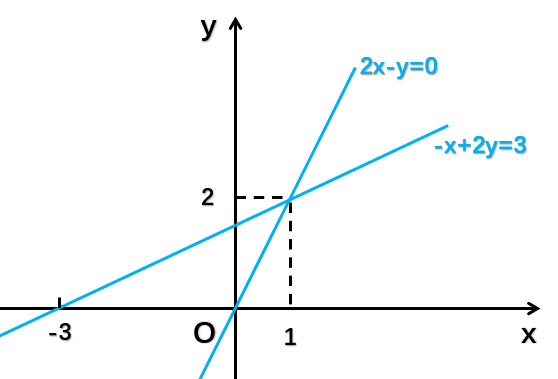
\includegraphics[width=0.4\textwidth]{figures/S1-1.png}
\end{center}
{\textcolor{anhao-purple}{to find the point that lies on both two lines}}
\newline
what's the {\textcolor{anhao-scarlet}{\bf{column}}} picture?
\newline
\begin{math}
x 
\begin{bmatrix}
	2 \\
	-1
\end{bmatrix}
+
y
\begin{bmatrix}
	-1 \\
	2
\end{bmatrix}
=
\begin{bmatrix}
	0 \\
	3
\end{bmatrix}
\end{math}
\begin{center}
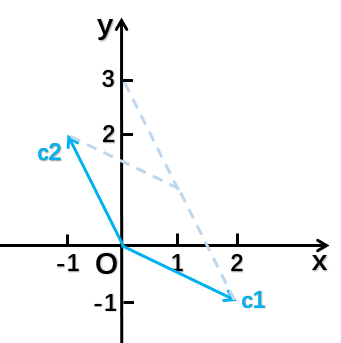
\includegraphics[width=0.3\textwidth]{figures/S1-2.png}
\end{center}
\begin{displaymath}
1{\overrightarrow{c_1}}+2{\overrightarrow{c_2}}={\overrightarrow{b}}
\end{displaymath}
{\textcolor{anhao-purple}{to find the linear combination of columns of {\bf{A}}, such that it equals {\bf{b}}}}
\vspace{14pt}
\newline
what linear combination gives {\bf{b}}?
\newline
what do all the linear combinations give?
\newline
what are all the possible, achievable right-hand sides be?
\vspace{14pt}
\newline
\begin{math}
\left\{  
\begin{array}{rclrclrclrcl}
	2x & - & y & & & = & 0 &{\bf{\textcolor{anhao-orange}{1}}}&\\
	-x & + & 2y & - & z & = & -1 &{\bf{\textcolor{anhao-orange}{2}}}&\\
	& -& 3y & + & 4z & = & 4 &{\bf{\textcolor{anhao-orange}{3}}}&
\end{array}  
\right.
\end{math}
\newline
\begin{math}
\left\{  
\begin{array}{rcl}
	&{\bf{\textcolor{anhao-orange}{1}}}&
\end{array}  
\right.
\end{math}
\quad : the plot of all the points that solve it are a plane
\newline
\begin{math}
\left\{  
\begin{array}{rcl}
	&{\bf{\textcolor{anhao-orange}{2}}}& \\
	&{\bf{\textcolor{anhao-orange}{3}}}&
\end{array}  
\right.
\end{math}
\quad : two planes meet at a line
\newline
\begin{math}
\left\{  
\begin{array}{rcl}
	&{\bf{\textcolor{anhao-orange}{1}}}& \\
	&{\bf{\textcolor{anhao-orange}{2}}}& \\
	&{\bf{\textcolor{anhao-orange}{3}}}&
\end{array}  
\right.
\end{math}
\quad : meet at a point
\newline
{\bf{A}} = 
\begin{math}
\begin{bmatrix}
	2  & -1 & 0 \\
	-1 & 2 & -1 \\
	0 & -3 & 4
\end{bmatrix}
\end{math}
, {\bf{b}} =
\begin{math} 
\begin{bmatrix}
	0 \\
	-1\\
	4
\end{bmatrix}
\end{math}
\vspace{14pt}
\newline
what's the {\textcolor{anhao-scarlet}{\bf{row}}} picture?
\newline
{\textcolor{anhao-purple}{to find out all the points that satisfy all the equations}}
\newline
what's the {\textcolor{anhao-scarlet}{\bf{column}}} picture?
\newline
\begin{math}
x
\begin{bmatrix}
	2 \\
	-1\\
	0
\end{bmatrix}
 + y
\begin{bmatrix}
	-1 \\
	2\\
	-3
\end{bmatrix}
 + z
\begin{bmatrix}
	0 \\
	-1\\
	4
\end{bmatrix}
 = 
\begin{bmatrix}
	0 \\
	-1\\
	4
\end{bmatrix}
\end{math}
\vspace{14pt}
\newline
can I always solve {\bf{A}}{\bf{x}} = {\bf{b}} for every right-hand side {\bf{b}}?
\newline
do the linear combinations of the columns fill 3-dimensional space?
\newline
{\textcolor{anhao-purple}{for this {\bf{A}}, the answer is {\bf{YES}} (non-singular, invertible)}}
\newline
{\textcolor{anhao-purple}{but for some others {\bf{A}}, the answer could be {\bf{NO}} (singular, not-invertible)}}
\vspace{14pt}
\newline
if the 3 columns all lie in the same plane, 
\newline
so I could solve it for some right-hand sides, when ${\overrightarrow{b}}$ is in the plane,
\newline
but most right-hand sides would be out of the plane and unreachable.
\vspace{14pt}
\newline
in some case, the combinations of {\bf{n}} columns can only fill out {\bf{m}}-D (m < n)
\vspace{14pt}
\newline
\begin{math}
\begin{bmatrix}
	2 & 5 \\
	1 & 3 
\end{bmatrix}
\begin{bmatrix}
	1 \\
	2 
\end{bmatrix}
 = 
1
\begin{bmatrix}
	2 \\
	1 
\end{bmatrix}
 + 
2
\begin{bmatrix}
	5 \\
	3 
\end{bmatrix}
 = 
\begin{bmatrix}
	12 \\
	7 
\end{bmatrix}
\end{math}
\newline
{\bf{A}}{\bf{x}} means: {\bf{A}}{\bf{x}} is a combination of columns of {\bf{A}}
\end{document}